\def\Ponderation{33,33}
\def\SigleNumero{STT-1920}
\def\NomCours{Méthodes statistiques}
\def\DateEvaluation{11 février 2026}
\def\HeureEvaluation{13 h 30 à 15 h 20}
\def\Session{}
\def\NomEvaluation{Examen 1}

% Ne rien mettre entre les accolades si l'enseignant (ou l'enseignante) est aussi le coordonnateur (ou la coordonnatrice)
\def\Coordonnatrice{}
\def\Coordonnateur{}

% Ne rien mettre entre les accolades s'il y a plus d'une section
\def\Enseignant{Julien Miron}
\def\Enseignante{}

% Ne rien mettre entre les accolades s'il s'agit d'un cours à section unique
% Mettre le nom de chacun des enseignants et enseignantes entre les accolades
% Une case à cocher sera générée pour chacune des sections
\def\SectionA{}
\def\SectionB{}
\def\SectionC{}
\def\SectionD{}


\def\Directives{
\begin{enumerate}
\item Matériel autorisé:
\begin{itemize}
\item Calculatrice scientifique {\bf autorisée par la faculté des sciences et de génie};
\item Votre aide-mémoire d'une feuille recto-verso, écrit à la main.
\end{itemize}
\item Assurez-vous que cette évaluation comporte \numquestions ~exercices répartis sur \numpages{}~pages, pour un total de \numpoints{}~points.\
\item \textbf{Veuillez ne pas dégrafer votre examen.}
\item Vous devez\textbf{ justifier toutes vos réponses} par une démarche claire, sauf pour les questions à choix de réponse.\
\item Pour les questions à choix de réponse et les vrais ou faux, vous pouvez mettre un X, un crochet ($\checkmark$) ou remplir la case.\
\item Vous devez laisser tout ce qui ne servira pas durant l'examen à l'avant de la salle AVANT de rejoindre votre place.\
\item Vous n'avez droit à AUCUN appareil électronique en votre possession durant l'examen.
\item Une fois assis à votre place, vous devez demandez l'autorisation pour vous lever, même si l'examen n'est pas encore commencé.
\item Dans les 5 dernières minutes de l'examen, il sera interdit de se lever avant que TOUTES les copies n'aient été ramassées.
\end{enumerate}
\begin{itemize}
\item[$\rightarrow$] Le non-respect des consignes 7-8-9 entraînera une pénalité de 10\%.
\end{itemize}
}

\newcommand{\affichepoints}{}     % ← AVEC points
% \renewcommand{\affichepoints}{on} % ← SANS points (non vide)

\documentclass{Evaluation}
\usepackage{multicol,graphicx}

\printanswers



\begin{document}

\pageblanche

%%%%%%%%%%%%%%%% QUESTION %%%%%%%%%%%%%%%%
\begin{questions}

\question[3]\label{hist}
L'histogramme ci-dessous représente la quantité de nourriture sèche ingérée en une journée  par 40 vaches choisies au hasard dans un élevage de 360 vaches. \\



\begin{center}

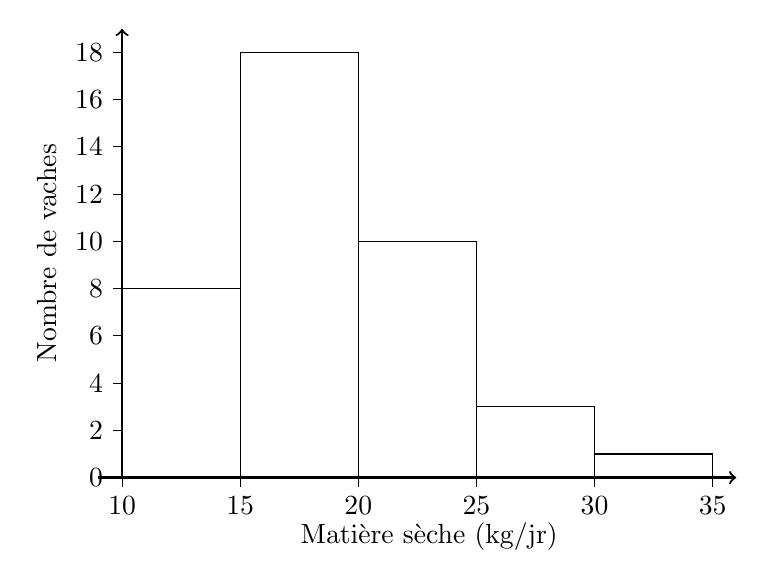
\begin{tikzpicture}[x=0.3cm,y=0.3cm]

% -------------------------------------------------
% Axes
% -------------------------------------------------
\draw[->, thick] (9,0) -- (36,0);   % axe x
\draw[->, thick] (10,0) -- (10,19); % axe y

% -------------------------------------------------
% Graduations x
% -------------------------------------------------
\foreach \x in {10,15,20,25,30,35}
  \draw (\x,0) -- (\x,-0.4) node[below] {\x};

% -------------------------------------------------
% Graduations y
% -------------------------------------------------
\foreach \y in {0,2,4,6,8,10,12,14,16,18}
  \draw (10,\y) -- (9.6,\y) node[left] {\y};

% -------------------------------------------------
% Labels
% -------------------------------------------------
\node at (23,-2.5) {Matière sèche (kg/jr)};
\node[rotate=90] at (6.8,9.5) {Nombre de vaches};

% -------------------------------------------------
% Histogramme (rectangles)
% Classes : [10,15[, [15,20[, [20,25[, [25,30[, [30,35[
% Effectifs : 8, 18, 10, 3, 1
% -------------------------------------------------
\draw (10,0) rectangle (15,8);
\draw (15,0) rectangle (20,18);
\draw (20,0) rectangle (25,10);
\draw (25,0) rectangle (30,3);
\draw (30,0) rectangle (35,1);

\end{tikzpicture}
\end{center}


De quel type de variable s'agit-il? 
 

	
\begin{checkboxes}
        \choice Quantitative discrète
        \correctchoice Quantitative continue
        \choice Qualitative nominale
        \choice Qualitative ordinale
	\end{checkboxes}

\begin{solution}
La quantité ingérée est une mesure en kg/jr, donc une variable quantitative continue.
\end{solution}


\question[3] En utilisant l'histogramme de l'exercice \ref{hist}, dans quelle classe de l'histogramme se situe le quantile d'ordre 0,30?

	\begin{checkboxes}
        \choice Dans la classe [10,15[
        \correctchoice Dans la classe [15,20[
        \choice Dans la classe [20,25[
        \choice Dans la classe [25,30[
        \choice Dans la classe [30,35]
	\end{checkboxes}

\begin{solution}
Le quantile 0,30 est la 12e observation ($0,30\times 40$). Les 8 premières sont dans [10,15[, la 12e est donc dans [15,20[.
\end{solution}


\question[3] Quel énoncé est vrai parmi les suivants?

\begin{checkboxes}
    \choice La somme des probabilités de deux événements mutuellement exclusifs peut être plus grande que 1.
    \correctchoice La somme des probabilités de deux événements qui ne sont pas mutuellement exclusifs peut être plus grande que 1.
    \choice Si la somme des probabilités de deux événements égale 1, nous savons qu'il n'y a aucune autre possibilité que ces deux événements.
    \choice Un événement n'est pas nécessairement mutuellement exclusif avec son complément.
\end{checkboxes}

\begin{solution}
Si deux événements se recouvrent, on peut avoir $P(A)+P(B)>1$. Les autres énoncés sont faux.
\end{solution}

\pageblanche
\question\label{sang} Héma-Québec nous fournit les informations suivantes par rapport aux groupes sanguins:



\begin{table}[h]
    \centering
\begin{tabular}{|c|c|}
\hline
    Groupe & Proportion\\
    \hline
     A&  0,43\\
     B& ?\\
     AB& 0,03 \\
     O& 0,46\\
     \hline
\end{tabular}
    \label{tab:my_label}
\end{table}

Notez que AB est un groupe en soi, ce n'est pas une combinaison des groupes A et B. De plus, un individu ne peut pas avoir plus d'un groupe sanguin et il n'y a aucun autre groupe que les quatre mentionnés dans le tableau.


\begin{parts}

\part[6] Vous allez passer un test pour connaître votre groupe sanguin. Quelle est la probabilité que vous apparteniez au groupe B ou au groupe O ?

\begin{solution}
La proportion manquante est $P(B)=1-0,43-0,03-0,46=0,08$. Donc $P(B\cup O)=0,08+0,46=0,54$.
\end{solution}

\vspace{9cm}
\end{parts}
Pour ce qui suit, on utilise la variable aléatoire $X$, qui prend la valeur $1$ si un individu appartient au groupe sanguin A et $0$, s'il appartient à un autre groupe, et la variable aléatoire Y, qui compte le nombre d'individus parmi 10 qui appartiennent au groupe sanguin A.
\begin{parts}
\setcounter{partno}{2}
\part[3] Quelle est la loi de $X$ ?
\begin{solution}
$X$ suit une loi de Bernoulli de paramètre $p=0,43$.
\end{solution}
\vspace{3.5cm}
\part[3] Quelle est la loi de $Y$ ?
\begin{solution}
$Y$ suit une loi binomiale $\text{Binomiale}(n=10, p=0,43)$.
\end{solution}
\end{parts}

\pageblanche
\question Le nombre de naissances quotidiennes dans un certain centre d’obstétrique suit une loi de Poisson de paramètre $\lambda=8$.
\medskip
\begin{parts}
\part[6] Quelle est la probabilité qu'il y ait 3 naissances ou plus dans ce centre lors d'un jour donné.

\begin{solution}
Si $N\sim\text{Poisson}(8)$, alors $P(N\ge 3)=1-P(N\le 2)=1-e^{-8}(1+8+32)=1-41e^{-8}\approx 0,9863$.
\end{solution}

\vspace{13cm}
\end{parts}
Une infirmière inscrit chaque jour le nombre de naissances dans un fichier Excel, durant une année.
\begin{parts}
\setcounter{partno}{1}
\part[2] On s'attend à ce que la moyenne de ces 365 observations soit environ égale à quelle valeur?

\begin{solution}
La moyenne attendue d'une observation est $\lambda=8$, donc la moyenne des 365 jours est environ $8$.
\end{solution}

\vspace{1cm}

\part[2] On s'attend à ce que la variance de ces 365 observations soit environ égale à quelle valeur?

\begin{solution}
Pour une loi de Poisson, la variance vaut $\lambda=8$. On s'attend donc à environ $8$.
\end{solution}

\end{parts}

\pageblanche
\question[3] Deux futurs parents sont porteurs du génotype Aa, où «A» est l'allèle dominante et «a» est l'allèle récessive. À chaque grossesse, la probabilité de donner naissance à un enfant porteur de l'allèle dominante est de 75 \% et chacune des naissances est indépendantes des autres. Ce couple prévoit avoir 4 enfants. Soit les événements $W$:«Le deuxième enfant n'est pas porteur de l'allèle dominante» et $Y$:«Exactement trois des quatre enfants du couple sont porteurs de l'allèle dominante». Quelles sont les probabilités associées à ces deux événements?

\begin{checkboxes}
\correctchoice $P(W)=0,25$ et $P(Y)\approx 0,422$
\choice $P(W)=0,25$ et $P(Y)\approx 0,047$
\choice $P(W)=0,75$ et $P(Y)\approx 0,422$
\choice $P(W)=0,75$ et $P(Y)\approx 0,047$
\end{checkboxes}
\vspace{0.5cm}
 


\begin{solution}
$P(W)=0,25$ et $P(Y)=\binom{4}{3}(0,75)^3(0,25)\approx 0,4219$.
\end{solution}


\question


\begin{parts}
\part[2] Si X suit une loi normale
$\mathcal{N}(8, 25)$, nous avons: $P(X\leq 13)=P(Z\leq \frac{13-8}{5})=\Phi(\frac{13-8}{5})$, où $Z\sim\mathcal{N}(0,1)$.

\begin{oneparcheckboxes}
    \correctchoice Vrai 
    \choice Faux
\end{oneparcheckboxes} \vspace{0.5cm}

\begin{solution}
On standardise : $Z=(X-8)/5$, donc $P(X\le 13)=P(Z\le 1)=\Phi(1)$.
\end{solution}

\part[2] Deux événements A et B sont mutuellement exclusifs si et seulement si A et B sont indépendants.

 \begin{oneparcheckboxes}
    \choice Vrai 
    \correctchoice Faux
\end{oneparcheckboxes} \vspace{0.5cm}

\begin{solution}
L'exclusivité donne $P(A\cap B)=0$, l'indépendance exige $P(A\cap B)=P(A)P(B)$. Les deux ne coïncident que si $P(A)=0$ ou $P(B)=0$.
\end{solution}

\part[2] Si $R$ et $S$ sont deux événements indépendants, alors nous avons toujours $P(R\cup S)=P(R)P(S)$.

 \begin{oneparcheckboxes}
    \choice Vrai 
    \correctchoice Faux
\end{oneparcheckboxes} \vspace{0.5cm}

\begin{solution}
La formule correcte est $P(R\cup S)=P(R)+P(S)-P(R)P(S)$.
\end{solution}

\part[2] Le coefficient binomial $\displaystyle {M \choose j}$ nous donne la probabilité de choisir $j$ éléments différents parmi $M$ éléments possibles.

 \begin{oneparcheckboxes}
    \choice Vrai 
    \correctchoice Faux
\end{oneparcheckboxes} \vspace{0.5cm}

\begin{solution}
${M \choose j}$ compte le nombre de combinaisons possibles, ce n'est pas une probabilité.
\end{solution}

\part[2] Si $X$ a une fonction de densité symétrique, alors nous sommes certains qu'il s'agit de la loi normale.

 \begin{oneparcheckboxes}
    \choice Vrai 
    \correctchoice Faux
\end{oneparcheckboxes} \vspace{0.5cm}

\begin{solution}
Plusieurs lois ont une densité symétrique (ex. uniforme), sans être normale.
\end{solution}

\part[2] Il est toujours possible d'identifier le minimum, la médiane et le maximum d'un échantillon sur un diagramme en boîte.

 \begin{oneparcheckboxes}
    \correctchoice Vrai 
    \choice Faux
\end{oneparcheckboxes} \vspace{0.5cm}

\begin{solution}
Un diagramme en boîte standard affiche le minimum, la médiane et le maximum de l'échantillon.
\end{solution}

\part[2] On répète 12 fois de façon indépendante une épreuve de Bernoulli dont la probabilité de succès est de 0,80. Alors on peut dire que le nombre de succès suit une loi $\text{Binomiale}(n = 12, p = 0,8)$ et que le nombre d’échecs suit une loi $\text{Binomiale}(n = 12, p = 0,2)$.

 \begin{oneparcheckboxes}
    \correctchoice Vrai 
    \choice Faux
\end{oneparcheckboxes} \vspace{0.5cm}

\begin{solution}
Le nombre de succès suit $\text{Binomiale}(12,0,8)$ et le nombre d'échecs suit $\text{Binomiale}(12,0,2)$ (ou $12-$succès).
\end{solution}

\end{parts}

\newpage
\question On suppose que la pression artérielle systolique (en mm Hg) suit une loi normale de moyenne 133 et de variance $6^2$. On utilisera $X$ pour dénoter cette variable aléatoire. Donc $X\sim\mathcal{N}(133, 6^2)$.

\begin{parts}
\part[3] Quelle est la probabilité qu'un individu choisi au hasard ait une pression artérielle systolique inférieure ou égale à 133? Justifiez votre réponse!

\begin{solution}
Par symétrie de la loi normale, $P(X\le 133)=0,5$.
\end{solution}

\vspace{3cm}

\part[8] Nous aimerions connaître la probabilité qu'un individu choisi au hasard ait une pression artérielle systolique inférieure à 124 ou supérieure à 139. Calculez cette probabilité en utilisant la table de la loi normale de la page précédente. Utilisez 4 chiffres après la virgule dans vos calculs et dans votre réponse.  
\begin{solution}
$z_1=(124-133)/6=-1,5$ et $z_2=(139-133)/6=1,0$. Donc $P(X<124)+P(X>139)=\Phi(-1,5)+[1-\Phi(1,0)]=0,0668+0,1587=0,2255$.
\end{solution}

\vspace{13cm}

\part[4] Si on prenait un échantillon de 100 personnes, quelle serait la variance de la moyenne échantillonnale $\overline{X}$? Donnez la valeur de cette variance!  

\begin{solution}
$\mathrm{Var}(\overline{X})=\sigma^2/n=36/100=0,36$.
\end{solution}

\end{parts}

\pageblanche

\question Une association agricole évalue qu'une brebis adulte coûte en moyenne 80\$ par année à nourrir, avec un écart-type de 12\$. Voici les diagrammes de la fonction de densité et de la fonction de répartition du modèle probabiliste supposé.

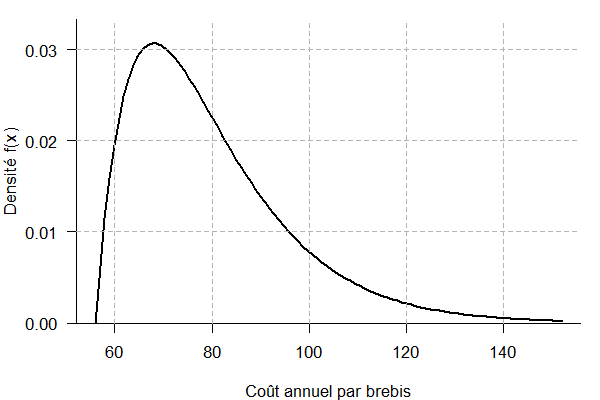
\includegraphics[width=8cm]{chi-den.png}
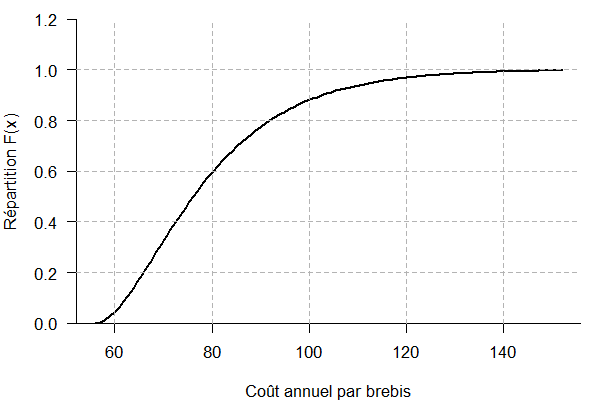
\includegraphics[width=8cm]{chi-rep.png}

\begin{parts}
\part[2] En utilisant les diagrammes, quelle est la probabilité approximative que le coût annuel par brebis soit suppérieur à 80\$ ?

\begin{solution}
D'après la fonction de répartition, $F(80)\approx 0,6$, donc $P(X>80)\approx 1-0,6=0,4$.
\end{solution}

\vspace{2cm}

\part[2] En utilisant les diagrammes, dites si la loi normale convient pour modéliser cette variable aléatoire. Donnez au moins une raison!

\begin{solution}
Non, la densité n'est pas symétrique (asymétrie à droite), ce qui va à l'encontre d'une loi normale.
\end{solution}

\vspace{1.5cm}

\part[8] Une ferme possède un élevage de 400 brebis. Donnez une approximation de la probabilité que le montant annuel à débourser pour les nourrir dépasse 32120\$. 

\newpage

\begin{solution}
Par le TCL, la somme $S$ est approximativement normale avec $\mu=400\times 80=32000$ et $\sigma=12\sqrt{400}=240$. Ainsi $P(S>32120)\approx 1-\Phi((32120-32000)/240)=1-\Phi(0,5)\approx 0,3085$.
\end{solution}


\end{parts}

\question[5] Soit $A$ et $B$, deux événements pour lesquels $P(A\cap B)=0,25$, $P(A\cap \bar{B})=0,1$ et $P(B\cap \bar{A})=0,3$.

Que vaut $P(A\cup B)$?

\begin{solution}
$P(A\cup B)=P(A\cap B)+P(A\cap \bar{B})+P(B\cap \bar{A})=0,25+0,10+0,30=0,65$.
\end{solution}

\pageblanche
%
\includepdf[pages={1}]{Tables_lois.pdf}

\end{questions}
\end{document} 
